In this section, we evaluate our approximate posterior on another subimage of M2. Figure~\ref{fig:marked_m2} is an image of M2. In red is the subimage considered in the body of the paper. 
We ran the wake-sleep algorithm on the red region, and here, we examine the results on the blue image. 


\begin{figure}
    \centering
    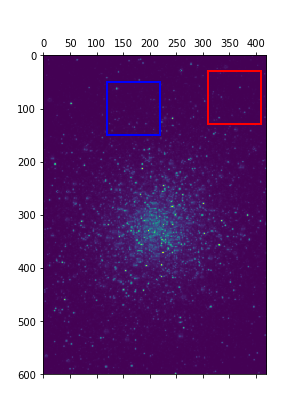
\includegraphics{figures/sdss_m2_image2_marked.png}
    \caption{An image of M2. We trained the wake-sleep algorithm on the red subregion, and evaluated our variational posterior in the blue region. }
    \label{fig:marked_m2}
\end{figure}

\begin{figure}[ht]
\begin{subfigure}{\textwidth}
\centering
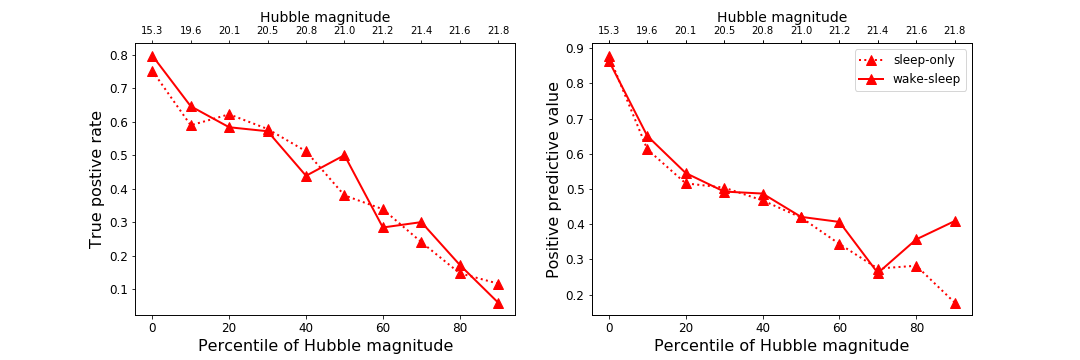
\includegraphics[width = \textwidth]{figures/summary_statistics_m2_alt.png}
\end{subfigure}
\begin{subfigure}{\textwidth}
\begin{center}
\begin{tabular}{lrrr}
\toprule
 &   TPR &   PPV &  F1 score  \\
\midrule
 Sleep-only &  0.51 &  0.47 &      0.49 \\
 Wake-sleep &  0.49 &  0.64 &      0.56  \\
Sleep-only (test) &  0.43 &  0.45 & 0.44 \\
 Wake-sleep (test) &  0.40 &  0.53 &      0.45  \\
\bottomrule
\end{tabular}
\par\vspace{0pt}
\end{center}
\end{subfigure}\hfill
\caption{Results on the test region of M2. }
\end{figure}
